\documentclass[a4paper,12pt]{report}
\usepackage{alltt, fancyvrb, url}
\usepackage{graphicx}
\usepackage[utf8]{inputenc}
\usepackage{float}
\usepackage{hyperref}
\usepackage{minted}
\graphicspath{{./images}}

% Questo commentalo se vuoi scrivere in inglese.
\usepackage[italian]{babel}

\usepackage[italian]{cleveref}
\title{Relazione del progetto di Programmazione di Reti 
    \\ Traccia 1: Configurazione di una Rete con VLAN e Routing Inter-VLAN}

\author{Leonardo Grimaldi}
\date{\today}   
\begin{document}
\maketitle
\tableofcontents
\chapter{Consegna}
\section{Descrizione}
Gli studenti dovranno progettare e configurare una rete che include due LAN separate in due VLAN su GNS3, utilizzando switch e router virtuali. La configurazione richiederà il routing inter-VLAN per permettere la comunicazione tra le VLAN.
\section{Obiettivi}
Configurare VLAN, routing inter-VLAN, e verificare la connettività tra dispositivi su VLAN diverse.
\section{Consegne richieste}
Documentazione della configurazione, spiegazione dei comandi utilizzati e cattura del traffico di rete per dimostrare la comunicazione tra le VLAN.
\chapter{Progettazione}
L'Università di Bologna e il Politecnico di Torino 
La topologia di rete ideata è proposta nella figura \ref{fig:topologia_offline}. 
\begin{figure}
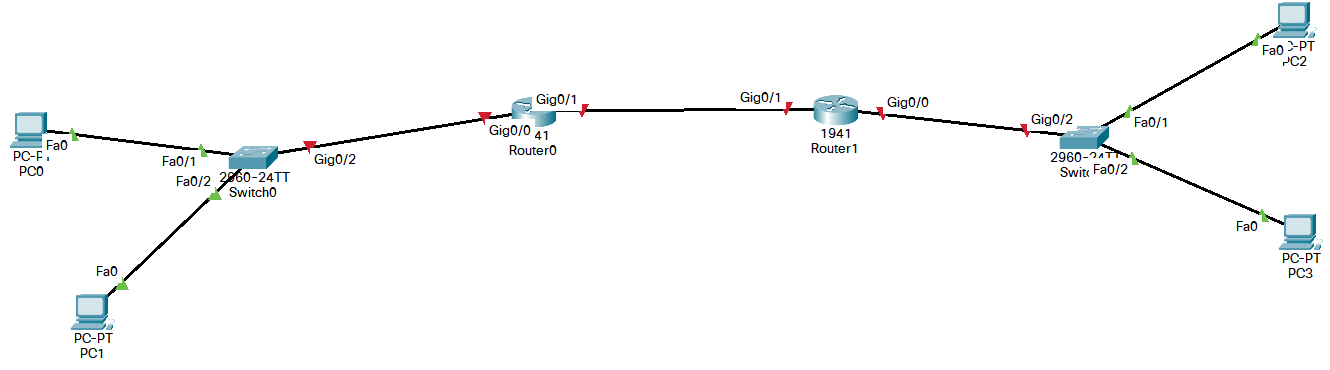
\includegraphics[width=\textwidth]{topology_offline.png}
\caption{Topologia offline}
\label{fig:topologia_offline}
\end{figure}
\chapter{Configurazione}
\end{document}